\section{Scratch}

\begin{figure}[H]
    \centering
    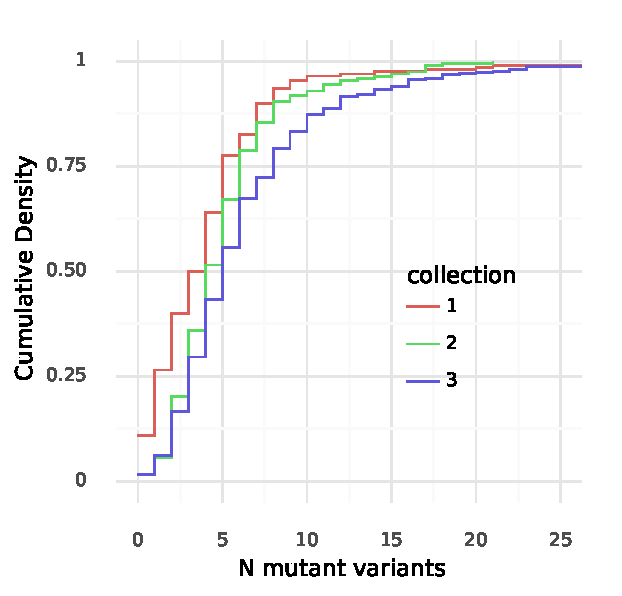
\includegraphics{figures/nvar_plot.pdf}
    \caption{Number of variants per sample}
    \label{fig:sample_nvar_counts}
\end{figure}


A place where old text goes before being forgotten.

\begin{enumerate}
	\item \subsection{Justification option 1: argument for excluding collection 3}
	\begin{enumerate}
	\item The sample size estimates in the study protocol for Sample Collection 3 did not take into account the 
	the effect of conditioning on LDT results. Thus, although the number of concordances and
	discordances matched what was expected during study design, the confidence intervals were much
	wider. The LLCIs dropped below some acceptance criteria.
	However, sample collections 1 and 2, the samples which Guardant did not select, had
	many positives to provide confidence in the results.
	\end{enumerate}
	
	\item \subsection{Justification option 2: incorrect combination of study collections}
	\begin{enumerate}
	\item The study protocol combines the PPA from each sample collection by a weighted sum
	of PPA values. The weights are the number of LBP70-positives. Since the third sample collection
	has the most LBP70-positives, it contributes the most to the combined PPA. However, the third
	sample collection also has the most uncertainty since there were so few LDT-negative
	samples. Therefore, an alternative variance-weighted strategy is more appropriate.
	\end{enumerate}
	
	\item \subsection{Justification option 3: an uncorrected bias, variants}
	\begin{enumerate}
	    \item On average, Guardant observes approximately three mutant variants for
	    each clinical sample. However, a small percentage of samples thirty or more
	    mutant variants. For example, when a germline
	    frameshift mutation is present, there tends to be many very low-MAF somatic 
	    frameshift mutations which revert the frameshift. These samples are rare
	    in the normal clinical population, but they were enriched in this accuracy
	    study and in some cases overwhelm the PPA and NPA values. Therefore, Guardant
	    calculated the prevalence of each clinical class and conditioned on the prior
	    frequencies to correct for this overrpresentation of samples with many variants.
	\end{enumerate}
	
	\item \subsection{Justification option 4: an argument for no bias correction}
	\begin{enumerate}
	    \item The study protocol conditions on LDT results based on the assumption
	    that samples which were previously detected by Guardant with the LDT test 
	    would have a higher chance 
	    of being detected again by Guardant with the CDx version of its test. 
	    The underlying principle for this assumption
	    is that sensitivity is driven by the number of ctDNA molecules in the tube of blood (or the
	    MAF). If a variant was detected by the LDT test, it is then more likely to have more
	    ctDNA molecules and in turn more likely to be detected by the CDx test. However,
	    the results of the study were that the MAFs were similar between all sample collections,
	    and so all sample collections should be analyzed in the same way. Therefore, 
	    PPA was calculated using only the MDL and CDx results for all sample collections.
	\end{enumerate}
	
	\item \subsection{Justification option 5: an uncorrected bias, molecules}
	\begin{enumerate}
	    \item Using the same arguments as ``Justification 4'', the more precise
	    variable to condition on is the number of molecules, not the presence or
	    absence of a call. This approach is a more refined method to correct for the bias.
	\end{enumerate}
	
	\item \subsection{Aaron's attempt to describe here the issue of overcorrection}
	\begin{enumerate}
    \item Given that the samples in
    sample collection 3 were selected based on results of the LDT version of the G360 test, there
    was a concern during study design that these samples would be biased such that the PPA
    performance would be overestimated. Therefore, a method was developed to correct this selection
    bias. However, the correction yielded larger than anticipated corrections (e.g. fusion PPA LLCI
    decreased from 91.5\% to 29.9\%). Something about the assumptions... In examining the PPA
    results from each sample selection cohort, the results appear comparable (e.g. X vs. Y)
    suggesting that the sample selection bias is less severe than anticipated. It is not possible
    to both have a study containing numerous variants of interest (many relatively rare) that
    represents an unbiased population. We do not know of a method to correct for the bias inherent
    in such a study, and therefore present the uncorrected PPA results.
    \end{enumerate}

	\item \subsection{Marcin's attempt to describe here the issue of overcorrection}
	\begin{enumerate}
    \item Under working assumption that the LDT and MDL tests have similar sensitivity,
    we would expect the unbiased population to have approximately equal probabilities of
    P(LDT+,MDL-) and P(LDT-,MDL+). The original bias model assumed enrichment for LDT+,
    which would have to translate to P(LDT+,MDL-) increasing relative to P(LDT-,MDL+).
    However collection 3 data shows no such increase.
    \end{enumerate}
    
    \item The combined PPA from all sample collections was calculated by summing
      all concordant variants between CDx and MDL divided by the number of total variants
      called positive by MDL. \cref{t:ppa_combined} shows the combined PPA when sample
      collection 3 is conditioned on LDT results (``Conditioned'') or when it is not
      (``Unconditioned'').  For CNVs, clinically relevant SNVs, and panel-wide SNVs, the
      LLCI of the combined PPA from all sample collections met the acceptance criteria
      (\cref{t:ppa_combined}).  For fusion calls, clinically relevant indels, and
      panel-wide indels, the LLCI of the PPA was below the estimated LLCI from the
      acceptance criteria in the protocol when the third sample collection was conditioned
      on LDT results.
      
    	\item \subsection{Summary results for each sample collections}
	
    	\captionsetup{width=.8\textwidth}
        \begin{table}[H]
        \centering
        \input{tables/ppa_summary_collections.tex}
        \caption[Summary of PPA for each sample collection]
        {\textbf{Summary of PPA for each sample collection.}}
        \label{t:ppa_summary_collections}
        \end{table}
    	
        \captionsetup{width=.8\textwidth}
        \begin{table}[H]
        \centering
        \input{tables/npa_summary_collections.tex}
        \caption[Summary of NPA for each sample collection]
        {\textbf{Summary of NPA for each sample collection.}}
        \label{t:npa_summary_collections}
        \end{table}
\end{enumerate}

Any way to preempt questions? Probably not.